\section{КЛАССИЧЕСКИЕ МЕТОДЫ ДЛЯ РЕШЕНИЯ ОДУ}

\subsection{Постановка задачи}

Программа, над которой ведётся работа, предназначена для решения дифференциальных уравнений или систем дифференциальных 
уравнений с начальными значениями, то есть задачи Коши ~--- классической математической постановки. 
Сама по себе задача достаточно сложная и изучалась уже более ста лет.

Конкретная прикладная задача сводится к решению дифференциального уравнения произвольного порядка \ref{eq-koshi}:
\begin{equation}
    \begin{cases}
        y^{(n)} = f(x, y, y', y'', ..., y^{(n - 1)})\\
        y(x_0) = y_0\\
        y'(x_0) = y_1\\
        y''(x_0) = y_2\\
        ...\\
        y^{(n - 1)}(x_0) = y_{n - 1}
    \end{cases}
    \label{eq-koshi}
\end{equation}

Данное уравнение произвольного порядка $n$ может быть преобразовано в систему из $n$ дифференциальных уравнений первого порядка путём
замены переменных. Пример \ref{eq-koshi-system} демонстрирует преобразование задачи Коши второго порядка в систему из 2-х уравнений
первого порядка, путём замены $y'$ на $z$:
\begin{equation}
    \begin{cases}
        z' = f(x, y, y', y'')\\
        y' = z\\
        y(x_0) = y_0\\
        z(x_0) = y_1
    \end{cases}
    \label{eq-koshi-system}
\end{equation}

Из курса дифференциальных уравнений известно, что задача с начальными условиями при непрерывных правых частях, удовлетворяющих условию
Липшица по всем переменным, имеет единственное решение.

Методы решения дифференциальных уравнений можно классифицировать на точные, приближенные и численные. Точные методы, которые изучаются
в курсе дифференциальных уравнений и могут быть применены к очень ограниченному кругу уравнений, позволяют выразить решение
дифференциальных уравнений либо через элементарные функции, либо с помощью квадратур от элементарных функций. К приближенным методам
относятся приемы, в которых решение дифференциального уравнения получается, как предел некоторой последовательности, элементы которой
построены с помощью элементарных функций. Численные методы представляют собой алгоритмы вычисления приближенных значений искомой
функции в узлах. %ссылку бы сюда

Такие задачи могут отличаться между собой сложностью решения. Так одни задачи можно решать при помощи группы явных методов и получать
достаточно точное решение. Другие же задачи, в которых присутствует резкий скачок градиента функции, решать приходится с использованием
неявных схем. Такие задачи называются жёсткими.

\subsection{Жёсткость}

Будем считать линейную систему обыкновенных дифференциальных уравнений $u' = Au$ ($A$ ~--- постоянная матрица $n \times n$)
жёсткой, если выполняются следующие требования:

\begin{enumerate}
    \item все собственные числа $\lambda_i$ матрицы $A$ имеют отрицательную действительную часть, т. е. $Re\lambda_i < 0$, 
    $i = 1, 2, ..., n$;
    \item число
        \begin{equation}
            S = \dfrac{\max\limits_{1 \leq k \leq n}|Re\lambda_k|}{\min\limits_{1 \leq k \leq n}|Re\lambda_k|}
            \label{eq:tough}
        \end{equation}
        велико
\end{enumerate}

Число \ref{eq:tough} называется жёсткостью задачи.

Для жёстких задач число жёсткости должно быть намного больше единицы, однако чёткой границы между жёсткой и нежёсткой задачей нет. Так
модельные уравнения с числом жёсткости более 100 уже дают небольшие скачки погрешности решения. В задачах химической кинетики число
жёсткости может быть более $10^6$.

\subsection{Явные схемы для решения ОДУ}

Для решения жёстких и нежёстких задач можно использовать различные семейства методов. В данной работе будет рассмотрено семейство
одношаговых методов Рунге-Кутты.

В семейство методов Рунге-Кутты входит огромное число схем, как явных, так и неявных. Все эти методы представлены в виде таблиц
Бутчера.

Явные методы обладают нижней диагональной формой таблицы Бутчера и позволяют решать задачи обычными маршевыми методами. В связи с тем,
что явные методы являются условно устойчивыми, работа с ними сильно зависит от размера шага итегрирования и для достижения заданной
точности требуют достаточно мелкий шаг интегрирования и повторного вычисления для повышения порядка точности процедурой Рунге-Ромберга.

%Общий вид явных схем:

% \begin{equation}
%     \begin{cases}
%         y_{k + 1} = y_k + \Delta y_k\\
%         \Delta y_k = \mathlarger{\sum}\limits_{i = 1}^{p}b_iK_i^k\\
%         K_i^k = hf\underset{i = 2, 3, ..., p}{(x_k + c_i h, y_k + h \mathlarger{\sum}\limits_{j = 1}^{i - 1}a_{ij}K_j^k)}
%     \end{cases}
%     \label{eq:explicit}
% \end{equation}

\begin{figure}
    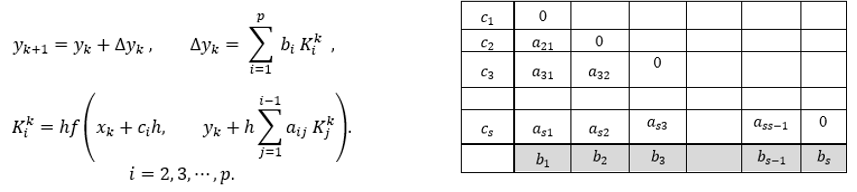
\includegraphics[width=15cm]{2-03-runge}
    \caption{Общий вид явных схем}
    \label{fig:runge}
\end{figure}

Примеры таблиц Бутчера для явных методов:

\begin{table}    
    \caption{Таблица Бутчера для метода явного метода Рунге-Кутты 4-го порядка}
    \begin{tabular}{|c|c|c|c|c|}
    \hline
    $0$ & $0$ & $0$ & $0$ & $0$\\
    \hline
    $\frac{1}{2}$ & $\frac{1}{2}$ & $0$ & $0$ & $0$\\
    \hline
    $\frac{1}{2}$ & $0$ & $\frac{1}{2}$ & $0$ & $0$\\
    \hline
    $1$ & $0$ & $0$ & $1$ & $0$\\
    \hline
    $0$ & \cellcolor{lightgray} $\frac{1}{6}$ & \cellcolor{lightgray} $\frac{1}{3}$ & \cellcolor{lightgray} $\frac{1}{3}$ & \cellcolor{lightgray} $\frac{1}{6}$\\
    \hline
    \end{tabular}
    \label{tab:RK4}
\end{table}

\begin{table}    
    \caption{Таблица Бутчера для метода явного метода Рунге-Кутты 6-го порядка}
    \begin{tabular}{|c|c|c|c|c|c|c|}
    \hline
    $0$ & $0$ & $0$ & $0$ & $0$ & $0$ & $0$\\
    \hline
    $\frac{1}{4}$ & $\frac{1}{4}$ & $0$ & $0$ & $0$ & $0$ & $0$\\
    \hline
    $\frac{1}{2}$ & $\frac{1}{2}$ & $0$ & $0$ & $0$ & $0$ & $0$\\
    \hline
    $\frac{1}{2}$ & $\frac{1}{7}$ & $\frac{2}{7}$ & $\frac{1}{14}$ & $0$ & $0$ & $0$\\
    \hline
    $\frac{3}{4}$ & $\frac{3}{8}$ & $0$ & $-\frac{1}{2}$ & $\frac{7}{8}$ & $0$ & $0$\\
    \hline
    $1$ & $-\frac{4}{7}$ & $\frac{12}{7}$ & $-\frac{2}{7}$ & $-1$ & $7$ & $0$\\
    \hline
    $0$ & \cellcolor{lightgray} $\frac{7}{90}$ & \cellcolor{lightgray} $\frac{16}{45}$ & \cellcolor{lightgray} $-\frac{1}{3}$ & \cellcolor{lightgray} $\frac{7}{15}$ & \cellcolor{lightgray} $\frac{16}{45}$ & \cellcolor{lightgray} $\frac{7}{90}$\\
    \hline
    \end{tabular}
    \label{tab:RK6}
\end{table}

\subsection{Явные вложенные схемы для решения ОДУ}

В связи с перечисленными недостатками обычных явных схем, есть смысл применить явные вложенные схемы, которые базируются так же на
нижней треугольной матрице Бутчера, обладают маршевым
методом решения и позволяют на базе одних и тех же поправочных коэффициентов моделировать решение с разным порядком точности и тем
самым либо увеличивать шаг интегрирования, либо уменьшать.

%(примеры таблиц Дормана-Принца и Фалберга 2)
%(формулы в общем виде)

\begin{figure}
    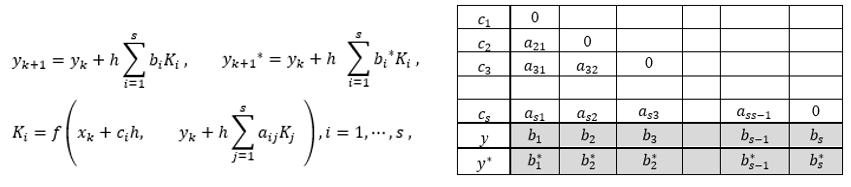
\includegraphics[width=15cm]{2-03-falberg}
    \caption{Общий вид явных вложенных схем}
    \label{fig:falberg}
\end{figure}

Примеры таблиц Бутчера для вложенных методов:

\begin{table}
    \caption{Таблица Бутчера для метода Фалберга 2-го порядка}
    \begin{tabular}{|c|c|c|c|}
    \hline
    $0$ & $0$ & $0$ & $0$\\
    \hline
    $1$ & $1$ & $0$ & $0$\\
    \hline
    $\frac{1}{2}$ & $\frac{1}{4}$ & $\frac{1}{4}$ & $0$\\
    \hline
    $0$ & \cellcolor{lightgray} $\frac{1}{2}$ & \cellcolor{lightgray} $\frac{1}{2}$ & \cellcolor{lightgray} $0$\\
    \hline
    $0$ & \cellcolor{lightgray} $\frac{1}{6}$ & \cellcolor{lightgray} $\frac{1}{6}$ & \cellcolor{lightgray} $\frac{4}{6}$\\
    \hline
    \end{tabular}
    \label{tab:Falberg2}
\end{table}

\begin{table}    
    \caption{Таблица Бутчера для метода Дормана-Принца 4-го порядка}
    \begin{tabular}{|c|c|c|c|c|c|c|c|}
    \hline
    $0$ & $0$ & $0$ & $0$ & $0$ & $0$ & $0$ & $0$\\
    \hline
    $\frac{1}{5}$ & $\frac{1}{5}$ & $0$ & $0$ & $0$ & $0$ & $0$ & $0$\\
    \hline
    $\frac{3}{10}$ & $\frac{3}{40}$ & $\frac{9}{40}$ & $0$ & $0$ & $0$ & $0$ & $0$\\
    \hline
    $\frac{4}{5}$ & $\frac{44}{45}$ & $-\frac{56}{15}$ & $\frac{32}{9}$ & $0$ & $0$ & $0$ & $0$\\
    \hline
    $\frac{8}{9}$ & $\frac{19372}{6561}$ & $-\frac{25360}{2187}$ & $\frac{64448}{6561}$ & $\frac{7}{8}$ & $0$ & $0$ & $0$\\
    \hline
    $1$ & $-\frac{4}{7}$ & $\frac{12}{7}$ & $-\frac{2}{7}$ & $-1$ & $7$ & $0$ & $0$\\
    \hline
    $0$ & \cellcolor{lightgray} $\frac{7}{90}$ & \cellcolor{lightgray} $\frac{16}{45}$ & \cellcolor{lightgray} $-\frac{1}{3}$ & \cellcolor{lightgray} $\frac{7}{15}$ & \cellcolor{lightgray} $\frac{16}{45}$ & \cellcolor{lightgray} $\frac{7}{90}$ & \cellcolor{lightgray} $0$\\
    \hline
    $0$ & \cellcolor{lightgray} $\frac{7}{90}$ & \cellcolor{lightgray} $\frac{16}{45}$ & \cellcolor{lightgray} $-\frac{1}{3}$ & \cellcolor{lightgray} $\frac{7}{15}$ & \cellcolor{lightgray} $\frac{16}{45}$ & \cellcolor{lightgray} $\frac{7}{90}$ & \cellcolor{lightgray} $0$\\
    \hline
    \end{tabular}
    \label{tab:DP4}
\end{table}

\subsection{Неявные схемы для решения ОДУ}

К наиболее сложным методам можно отнести группу неявных схем. Плотно заполненная таблица Бутчера не позволяет использовать маршевые
методы и принуждает решать систему алгебраических уравнений на каждом шаге интегрирования, что вызывет определённые сложности у
разработчиков.

%(примеры таблиц для двух неявных 4 и 6)
%(формулы в общем виде)
%(ссылки)

\begin{figure}
    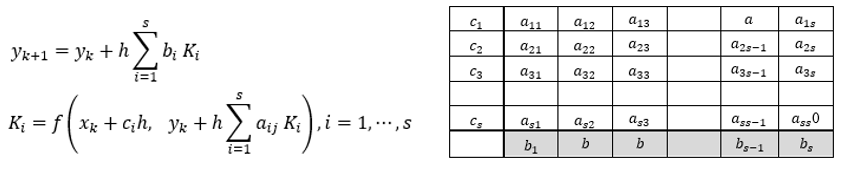
\includegraphics[width=15cm]{2-03-gauss}
    \caption{Общий вид неявных схем}
    \label{fig:gauss}
\end{figure}

Примеры таблиц Бутчера для неявных методов:

\begin{table}    
    \caption{Таблица Бутчера для метода неявного метода Гаусса 4-го порядка}
    \begin{tabular}{|c|c|c|c|c|}
    \hline
    $0$ & $0$ & $0$ & $0$ & $0$\\
    \hline
    $\frac{1}{2}$ & $\frac{1}{2}$ & $0$ & $0$ & $0$\\
    \hline
    $\frac{1}{2}$ & $0$ & $\frac{1}{2}$ & $0$ & $0$\\
    \hline
    $1$ & $0$ & $0$ & $1$ & $0$\\
    \hline
    $0$ & \cellcolor{lightgray} $\frac{1}{6}$ & \cellcolor{lightgray} $\frac{1}{3}$ & \cellcolor{lightgray} $\frac{1}{3}$ & \cellcolor{lightgray} $\frac{1}{6}$\\
    \hline
    \end{tabular}
    \label{tab:RK4}
\end{table}

\begin{table}    
    \caption{Таблица Бутчера для метода неявного метода Гаусса 6-го порядка}
    \begin{tabular}{|c|c|c|c|c|c|c|}
    \hline
    $0$ & $0$ & $0$ & $0$ & $0$ & $0$ & $0$\\
    \hline
    $\frac{1}{4}$ & $\frac{1}{4}$ & $0$ & $0$ & $0$ & $0$ & $0$\\
    \hline
    $\frac{1}{2}$ & $\frac{1}{2}$ & $0$ & $0$ & $0$ & $0$ & $0$\\
    \hline
    $\frac{1}{2}$ & $\frac{1}{7}$ & $\frac{2}{7}$ & $\frac{1}{14}$ & $0$ & $0$ & $0$\\
    \hline
    $\frac{3}{4}$ & $\frac{3}{8}$ & $0$ & $-\frac{1}{2}$ & $\frac{7}{8}$ & $0$ & $0$\\
    \hline
    $1$ & $-\frac{4}{7}$ & $\frac{12}{7}$ & $-\frac{2}{7}$ & $-1$ & $7$ & $0$\\
    \hline
    $0$ & \cellcolor{lightgray} $\frac{7}{90}$ & \cellcolor{lightgray} $\frac{16}{45}$ & \cellcolor{lightgray} $-\frac{1}{3}$ & \cellcolor{lightgray} $\frac{7}{15}$ & \cellcolor{lightgray} $\frac{16}{45}$ & \cellcolor{lightgray} $\frac{7}{90}$\\
    \hline
    \end{tabular}
    \label{tab:RK6}
\end{table}

Помимо перечисленных групп методов, существуют так же диагональные неявные методы, неявные вложенные, неявные методы без одной строки
или столбца



Диагональные неявные схемы (для сложных неработают)

Методы без одной строки или без одного столбца

Диагональные вложенные

УСТОЙЧИВОСТЬ


%Цитирование источника 4 \cite{Wikipedia4} \cite{cite_1_2} \cite{cite_1_15} \cite{cite_1_16}.
